\chapter{The Black - Scholes - Merton model}


\section{European Call Option Valuation}
\fontsize{11pt}{20pt}\selectfont Let $\{W_t : t\geq 0\}$ be a $\mathbb{P}$-standard Wiener process on the probability space ($\Omega$, $\mathcal{F}$, $\mathbb{P}$) and let the asset price $S_t$ follow a GBM with the following SDE \\
\begin{align*}
\dfrac{dS_t}{S_t}=\mu dt+\sigma dW_t
\end{align*}
where $\mu$ is the drift parameter and $\sigma$ is the volatility parameter. \\ \vspace{0.01cm}

We expected to express the time-t value $C(S_t, t)$ of a European call option following to the the Feynman-Kac formula, then $C(S_t, t)$ must be satisfied the equation (\refeq{eq5.3.1}). A European call option $C(S_t, t)$ which is described by It\=o' lemma is given by
\begin{align*}
dC(S_t, t)=\left(\dfrac{\partial C}{\partial t}+\mu_tS_t\dfrac{\partial C}{\partial S_t}+\dfrac{1}{2}\sigma^2 S_t^2\dfrac{\partial^2 C}{\partial S_t^2}\right)dt+\sigma_tS_t\dfrac{\partial C}{\partial S_t}dW_t
\end{align*}
Now consider  portfolio consisting of the call option and $\alpha$ stocks. Then the
cost of the portfolio is $C+\alpha S_t$. We get
\begin{align*}
d(C+\alpha S_t)=\left(\dfrac{\partial C}{\partial t}+\mu_tS_t\dfrac{\partial C}{\partial S_t}+\dfrac{1}{2}\sigma^2 S_t^2\dfrac{\partial^2 C}{\partial S_t^2}+\alpha\mu S_t\right)dt+\sigma_tS_t\left(\dfrac{\partial C}{\partial S_t}+\alpha\right)dW_t
\end{align*}
Now we let $\alpha=-\dfrac{\partial C}{\partial S_t}(S_t,t)$ to hedge away all risk in our portfolio.
\begin{align*}
d(C+\alpha S_t)=\left(\dfrac{\partial C}{\partial t}+\dfrac{1}{2}\sigma^2 S_t^2\dfrac{\partial^2 C}{\partial S_t^2}+\alpha\mu S_t\right)dt
\end{align*}
As one can see, the random component $dW_t$, is now gone. The portfolio has no risk, it must grow
over time at the risk-free rate $r$. Thus,
\begin{align*}
	\dfrac{d}{dt}(C+\alpha S_t)=r(C+\alpha S_t)=r(C-S_t\dfrac{\partial C}{\partial S_t})
\end{align*}
and
\begin{align*}
	r(C-S_t\dfrac{\partial C}{\partial S_t})dt=\left(\dfrac{\partial C}{\partial t}+\dfrac{1}{2}\sigma^2 S_t^2\dfrac{\partial^2 C}{\partial S_t^2}+\alpha\mu S_t\right)dt
\end{align*}
Rearranging gives us the result that $C(S_t, t)$ follows the Keynman-Kac formula
\begin{align*}
	\dfrac{\partial C}{\partial t}(S_t, t)+rS_t\dfrac{\partial C}{\partial S_t}+\dfrac{1}{2}\sigma^2S_t^2\dfrac{\partial^2C}{\partial S^2}(S_t, t)-rC=0
\end{align*}
This means that the time-t value $C(S_t, t)$ can be written as
\begin{align}
		C(S_t, t)=e^{-r(T-t)}\mathbb{E}^\mathbb{Q}[C (S_T, T)|\mathcal{F}_t] \label{eq5.5.1}
\end{align}
\indent A European call option $C(S_t; t)$ written on $S_t$ with strike
price $K$ has the payoff $C(S_T ; T) = \textnormal {max}(S_T-K; 0)$. We substitute this payoff
in the Feynman-Kac formula in Equation \eqref{eq5.5.1}. Hence, the time-$t$ value of a
European call is
\begin{align*}
	C(S_t,t;K,T) = e^{-r(T-t)}\mathbb{E}^\mathbb{Q}[\textnormal{max}\{S_T-K,0\}\mid\mathcal{F}_t]
\end{align*}
%where $\mathbb{E}^\mathbb{Q}$(.) is the expectation under the risk-neutral measure $\mathbb{Q}$.
%Using the risk-neutral valuation approach show that the European call option price is
%\begin{align*}
%	C(S_t,t;K,T)=S_te^{-(T-t)}\Phi(d_+)-Ke^{-r(T-t)}\Phi(d_-) 
%\end{align*} 
%where
%\begin{align*}
%d_\pm=\dfrac{\textnormal{log}(S_t/K)+(r-\pm \frac{1}{2}\sigma^2)(T-t)}{\sigma \sqrt{T-t}}
%\end{align*}
%and $\Phi(x)$ is the standard normal cdf
%\begin{align*}
%\Phi(x)=\displaystyle \int_{-\infty}^{x}\dfrac{1}{2\pi} e^{-\frac{1}{2}u^2}du
%\end{align*}
%
%Expain
From Girsanov's theorem, under a $\mathbb{Q}$-standard Wiener process we have
\begin{align*}
W_t^\mathbb{Q}&=W_t+\left(\dfrac{\mu-r}{\sigma}\right)t \hspace{0.2cm} 
\end{align*}
%This leads to
%\begin{align*}
%dW_t^\mathbb{Q}&=dW_t+\left(\dfrac{\mu-r}{\sigma}\right)dt
%\end{align*} 
% Hence, under the risk-neutral measure $\mathbb{Q}$ the asset price follows the diffusion process
%\begin{align*}
%\dfrac{dS_t}{S_t}&=\mu dt+\sigma\left(W_t^\mathbb{Q}-\dfrac{\mu-r}{\sigma}t\right)\\
%&=\mu dt+\sigma dW_t^\mathbb{Q}-(\mu-r)dt\\
%&=rdt+\sigma dW_t^\mathbb{Q}
%\end{align*}
And consider equation \eqref{eq2} which has been appoved in property of GBM
\begin{align*}
S_t=S_0e^{\left(\mu -\frac{1}{2}\sigma^2 \right)t+\sigma W_t}
\end{align*}
Under the risk-neutral measure $\mathbb{Q}$, that equation is equivalent to
\begin{align}
S_t=S_0e^{\left(r -\frac{1}{2}\sigma^2 \right)t+\sigma W_t^{\mathbb{Q}}} \label{eq5.5.2}
\end{align} 
where $r$ is the risk-free interest rate. This implies that
\begin{align*}
S_t&=e^{logS_0}e^{\left(r -\frac{1}{2}\sigma^2 \right)t+\sigma W_t^{\mathbb{Q}}}\\
&=e^{logS_0+\left(r -\frac{1}{2}\sigma^2 \right)t+\sigma W_t^{\mathbb{Q}}}
\end{align*}

For $T\hspace{0.1cm}>t\hspace{0.1cm}$, $W_{T-t}^\mathbb{Q} \sim \mathcal{N}(0, T-t)$. Hence, conditional on $S_t$ we can write
\begin{align*}
	S_T \mid S_t\sim \textnormal{log}-\mathcal{N}[\textnormal{log}S_t+(r-\dfrac{1}{2}\sigma^2)(T-t),\sigma^2(T-t)]
\end{align*}
Under the risk-neutral measure $\mathbb{Q}$ we can write the European call option price as
\begin{align*}
C(S_t,t;K,T) &= e^{-r(T-t)}\mathbb{E}^\mathbb{Q}[\textnormal{max}\{S_T-K,0\}\mid\mathcal{F}_t]\\
			&=e^{-r(T-t)} \displaystyle \int_{0}^{\infty}\textnormal{max}\{S_T-K,0\}f(S_T\mid S_t)dS_t.
\end{align*}
Here, for a log normally distributed random variable log $X\sim \mathcal{N}(\mu, \sigma^2)$ the PDF is
\begin{align*}
f_X(x; \mu, \sigma)=\dfrac{1}{x\sigma\sqrt{2\pi}}e^{-\frac{1}{2}\left(\frac{\log x-\mu}{\sigma}\right)^2} \hspace{0.2cm},\hspace{0.2cm} x\hspace{0.1cm} > \hspace{0.1cm}0
\end{align*}
Since $S_T$ conditional on $S_t$ have drift is equal to $\log S_t+(r-\dfrac{1}{2}\sigma^2)(T-t)$  
and we can thus write
\begin{align*}
f(S_T | S_t)=\dfrac{1}{S_T\sigma\sqrt{2\pi(T-t)}}e^{-\frac{1}{2}\left(\frac{\log S_T-\log S_t-(r-\frac{1}{2}\sigma^2)(T-t)}{\sigma\sqrt{T-t}}\right)^2} \hspace{0.2cm},\hspace{0.2cm} S_T\hspace{0.1cm} > \hspace{0.1cm}0
\end{align*}
or
\begin{align*}
f(S_T| S_t)=\dfrac{1}{S_T\sigma\sqrt{2\pi(T-t)}}e^{-\frac{1}{2}\left(\frac{\log S_T-m}{\sigma\sqrt{T-t}}\right)^2} \hspace{0.2cm},\hspace{0.2cm} S_T\hspace{0.1cm} > \hspace{0.1cm}0
\end{align*}
where $m=\log S_t+(r-\frac{1}{2}\sigma^2)(T-t)$. Therefore,
\begin{align*}
C(S_t,t;K,T) =\hspace{0.1cm} &e^{-r(T-t)} \displaystyle \int_{0}^{K}\max\{S_T-K,0\}f(S_T| S_t)dS_t \\ 		       &+e^{-r(T-t)} \displaystyle \int_{K}^{\infty}\max\{S_T-K,0\}f(S_T| S_t)dS_t\\
			  =\hspace{0.1cm} &e^{-r(T-t)} \displaystyle \int_{K}^{\infty}(S_T-K)f(S_T| S_t)dS_t\\
			  =\hspace{0.1cm} &I_1-I_2
\end{align*}
where
\begin{align*}
I_1=e^{-r(T-t)} \displaystyle \int_{K}^{\infty}S_Tf(S_T| S_t)dS_t \hspace{0.3cm} \textnormal{and} \hspace{0.3cm} I_2=e^{-r(T-t)} \displaystyle \int_{K}^{\infty}Kf(S_T| S_t)dS_t
\end{align*}
Solving $I_1$ we have 
\begin{align*}
I_1 &=e^{-r(T-t)} \displaystyle \int_{K}^{\infty}S_Tf(S_T\mid S_t)dS_t\\
	&=e^{-r(T-t)} \displaystyle \int_{K}^{\infty}\dfrac{1}{\sigma\sqrt{2\pi(T-t)}}e^{-\frac{1}{2}\left(\frac{\textnormal{log}S_T-m}{\sigma\sqrt{T-t}}\right)^2}dS_t
\end{align*}
and by letting $u=\frac{\log S_T-m}{\sigma\sqrt{T-t}}$ we then have
\begin{align*}
	I_1=\dfrac{e^{m-r(T-t)}}{\sqrt{2\pi}}\displaystyle \int_{\frac{\log K-m}{\sigma\sqrt{T-t}}}^{\infty}e^{-\frac{1}{2}u^2+\sigma u\sqrt{T-t}}du.
\end{align*}
Using the sum of squares
\begin{align*}
	-\dfrac{1}{2}u^2+\sigma u\sqrt{T-t}=\dfrac{1}{2}\left[(u-\sigma\sqrt{T-t})^2-\sigma^2(T-t)\right]
\end{align*}
we can simplify $I_1$ to become
\begin{align*}
I_1&=\dfrac{e^{m-r(T-t)}}{\sqrt{2\pi}}\displaystyle \int_{\frac{\log K-m}{\sigma\sqrt{T-t}}}^{\infty}e^{-\frac{1}{2}\left[(u-\sigma\sqrt{T-t})^2-\sigma^2(T-t)\right]}du\\
&=\dfrac{e^{m-r(T-t)+\frac{1}{2}\sigma^2(T-t)}}{\sqrt{2\pi}}\displaystyle\int_{\frac{\log K-m}{\sigma\sqrt{T-t}}}^{\infty}e^{-\frac{1}{2}\left(u-\sigma\sqrt{T-t}\right)^2}du\\
&=e^A\left[\displaystyle\int_{-\infty}^{\infty}\dfrac{1}{\sqrt{2\pi}}e^{-\frac{1}{2}\left(u-\sigma\sqrt{T-t}\right)^2}du-\displaystyle\int_{-\infty}^{\frac{\log K-m}{\sigma\sqrt{T-t}}}e^{-\frac{1}{2}\left(u-\sigma\sqrt{T-t}\right)^2}du\right]
\end{align*}
Where 
\begin{align*}
	A&=m-r(T-t)+\frac{1}{2}\sigma^2(T-t)\\
	&=\log S_t+(r-\frac{1}{2}\sigma^2)(T-t) -r(T-t)+\frac{1}{2}\sigma^2(T-t)=\log S_t
\end{align*}
By setting $v=u-\sigma\sqrt{T-t}=\dfrac{\log(K/S_t)-(r-\frac{1}{2}\sigma^2)(T-t)}{\sigma\sqrt{T-t}}$ and substituting\\ $m=\log S_t+(r+\frac{1}{2}\sigma^2)(T-t)$ we have
\begin{align*}
	\displaystyle\int_{-\infty}^{\frac{\log K-m}{\sigma\sqrt{T-t}}}e^{-\frac{1}{2}\left(u-\sigma\sqrt{T-t}\right)^2}du = \displaystyle\int_{-\infty}^{\frac{\log(K/S_t)-(r+\frac{1}{2}\sigma^2)(T-t)}{\sigma\sqrt{T-t}}}e^{-\frac{1}{2}\nu^2}d\nu
\end{align*}
Therefore, 
\begin{align*}
	I_1&=e^{\log S_t}\left[1-\displaystyle\int_{-\infty}^{\frac{\log(K/S_t)-(r+\frac{1}{2}\sigma^2)(T-t)}{\sigma\sqrt{T-t}}}e^{-\frac{1}{2}\nu^2}d\nu\right]\\
	&=S_t\left[1-\Phi\left(\dfrac{\log(K/S_t)-(r+\frac{1}{2}\sigma^2)(T-t)}{\sigma\sqrt{T-t}}\right)\right]\\
	&=S_t\Phi\left(\dfrac{\log(S_t/K)+(r+\frac{1}{2}\sigma^2)(T-t)}{\sigma\sqrt{T-t}}\right).
\end{align*}
Similarly for $I_2$ we have
\begin{align*}
 I_2&=e^{-r(T-t)} \displaystyle \int_{K}^{\infty}Kf(S_T)dS_T\\
 	&=Ke^{-r(T-t)} \displaystyle \int_{K}^{\infty}\dfrac{1}{S_T\sigma\sqrt{2\pi(T-t)}}e^{-\frac{1}{2}\left(\frac{\log S_T-m}{\sigma\sqrt{T-t}}\right)^2}dS_T
\end{align*}
and by letting  $u=\frac{\log S_T-m}{\sigma\sqrt{T-t}}$ and substituting $m=\log S_t+(r-\frac{1}{2}\sigma^2)(T-t)$ \\
\begin{align*}
I_2&=e^{-r(T-t)}K \displaystyle \int_{\frac{\log K-m}{\sigma\sqrt{T-t}}}^{\infty}\dfrac{1}{\sqrt{2\pi}}e^{-\frac{1}{2}u^2}du\\
	&=Ke^{-r(T-t)}\left[1-\Phi\left(\frac{\log K-m}{\sigma\sqrt{T-t}}\right)\right]\\
	&=Ke^{-r(T-t)}\left[1-\Phi\left(\dfrac{\log(K/S_t)-(r-\frac{1}{2}\sigma^2)(T-t)}{\sigma\sqrt{T-t}}\right)\right]\\
	&=Ke^{-r(T-t)}\Phi\left(\dfrac{\log(S_t/K)+(r-\frac{1}{2}\sigma^2)(T-t)}{\sigma\sqrt{T-t}}\right)
\end{align*}
Therefore, 
\begin{align}
	C(S_t,t;K,T)=S_te^{-(T-t)}\Phi(d_1)-Ke^{-r(T-t)}\Phi(d_2) \label{eqBS}
\end{align}
where 
\begin{align*}
d_1&=\dfrac{\log(S_t/K)+(r+ \frac{1}{2}\sigma^2)(T-t)}{\sigma \sqrt{T-t}}\\
d_2&=\dfrac{\log(S_t/K)+(r- \frac{1}{2}\sigma^2)(T-t)}{\sigma \sqrt{T-t}}
\end{align*}

\section{Application}

\subsection{Condition of the Black-Sholes-Merton moldel}
Six assumptions of the Black-Sholes-Merton model is given by
\begin{enumerate}
	\item The option is European 
	\item No dividends are paid out during the option's life
	\item Efficient markets
	\item There are no transaction costs in buying the option
	\item The risk-free rate and volatility of the underlying are known and constant
	\item The returns on the underlying are normally distributed
\end{enumerate}
\subsubsection*{Problem}
Consider a European call option on FPT stock without dividends. Market movements cannot be predicted. These information is given $5$ first assumptions. We need to check the last one which is the rate of returns are normally distributed. We can get the historical data from source: \url{http://www.cophieu68.vn/historyprice.php?id=fpt}, the stock price is just calculated in 1  year, 2017. Firstly, we will compute daily return $(u_i) $ of FPT stock. 
\begin{align*}
	u_i=\ln\dfrac{S_i}{S_{i-1}} \hspace{0.4cm} \text{for}\hspace{0.2cm}i=0, 1, \dots, n
\end{align*}
where \\
$n+1$: Number of observations\\
$S_i$: Stock price at end of $i$th interval, with $i=0, 1, \dots, n$
\subsubsection*{Testing for normal distribution}
The software is using for testing data is R – Studio. The code is shown at the end of report. We will use graphical methods which is normal probability plot (Q-Q plot or quantile quantile plots).
Q-Q plot is a graphical technique to help us assess whether or not a data set is approximately normally distributed. %The question is how to make a Q-Q plot. The method is following  
%\begin{itemize}
%	\item Sort the numbers from smallest to largest
%	\item Draw a normal distribution curve
%	\item Find the Z-value for each segment
%	\item Plot data set value against the Z-value 
%\end{itemize}
If the most part the data points follow along the straight line, this will be normally distributed. We will describe the previous daily return.  Here is our result
\begin{figure}[htp]
	\begin{center}
		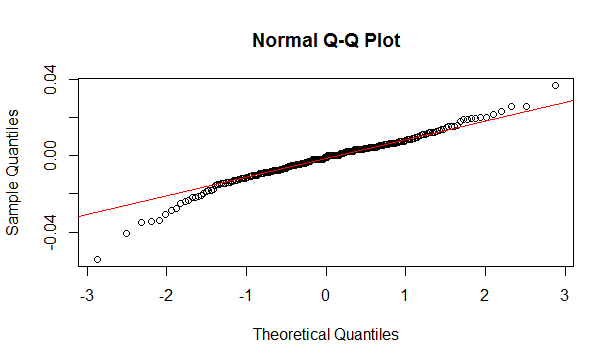
\includegraphics[scale=.8]{Rplot03}
	\end{center}
	\label{refRplot03}
	\caption{The distribution of FPT stock}
\end{figure}

\newpage
This graph satisfies conditions of normal distribution. Here the x-axis is the probability and the y-axis is the values of returns.
Therefore, the returns is most likely normally distribution.
\subsection{Apply to the Black-Scholes-Merton model}

Let's asumme that FPT stock satisfies conditions of the Black-Scholes-Merton model. We first estimate the volatility of a stock price empirically. The usual estimate, $s$, of the standard deviation of the $u_i$ is given by
\begin{align*}
	s&=\sqrt{\dfrac{1}{n-1}\sum_{i=1}^{n}(u_i-\bar{u})^2}
\end{align*}
or
\begin{align*}
 s=\sqrt{\dfrac{1}{n-1}\sum_{i=1}^{n}u_i^2-\dfrac{1}{n(n-1)}\left(\sum_{i=1}^{n}u_i\right)^2}
\end{align*}
where $\bar{u}$ is the mean of the $u_i$. An estimate for the volatility per annum as 
\begin{align*}
	\text{Volatility
	per annum} = \text{Volatility
	per trading day} \times \sqrt{\text{Number of trading days
		per annum}}
\end{align*}

\newpage
Using R-studio, we get 
\begin{itemize}
	\item Volatility
	per trading day $s = 0.015$
	\item There are 250 trading days of year 2017. Therefore,\\ Volatility
	per annum = $s\times \sqrt{250}$ = 24\%
\end{itemize}
This company currently sells for $59.8$ VND per share. The annual stock price volatility is $24\%$. Assume that the annual continuously compounded risk-free interest rate is $3\%$. Using the Black-Scholes model for the price of a call option on a company's stock with strike price $62$ VND and time for expiration of half a year. Let's cover it.
\begin{table}[!htp]
	\centering
	\begin{tabular}{|l|c|r|}
	\hline
	$S_0$ & Stock price at time zero   & $59.8$ VND\\
	\hline
	$K$ & Strike price  & $62$ VND\\
	\hline
	$\sigma$ &  Annual volitility & $24\%$\\
	\hline
	$r$ & Annual riskless rate  & $3\%$ \\
	\hline
	$T$ & Option expiration (in years)  & $0.5$\\
	\hline	
	\end{tabular}
	\caption{FPT stock}
	\label{B3.1}
\end{table}

We first calculate each components of equation \refeq{eqBS}. 
\begin{align*}
	d_1&=\dfrac{\log(S_0/K)+(r+ \frac{1}{2}\sigma^2)T}{\sigma \sqrt{T}}= -0.04\\
	d_2&=\dfrac{\log(S_0/K)+(r- \frac{1}{2}\sigma^2)T}{\sigma \sqrt{T}}=-0.21
\end{align*}
Substituting the above variables into equation \refeq{eqBS}, we get
\begin{align*}
	C(S_0,0;K,T)=S_0e^{-T}\Phi(d_1)-Ke^{-rT}\Phi(d_2)=3.48 
\end{align*}
This means that the option price or a premium is $3.48$ VND for each stock.